% The four TikZ figures drawn inline in the thesis LaTeX source, copied verbatim
% so they can be rendered as PNGs for the study guide.
% Build: pdflatex tikz_figures.tex  then  pdftoppm -r 220 -png tikz_figures.pdf tikz
\documentclass[tikz,border=10pt,12pt]{standalone}
\usepackage[T1]{fontenc}
\usepackage{lmodern}
\usepackage{amsmath}
\usetikzlibrary{shapes.geometric, arrows, positioning, fit}
\begin{document}

% 1. Three outcomes of approximate unlearning (Chapter 1)
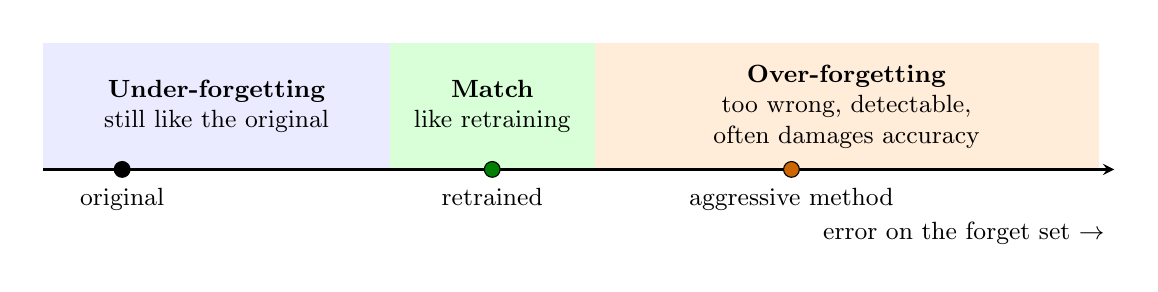
\begin{tikzpicture}[x=1cm,y=1cm]
    \fill[white] (-0.2,-1.2) rectangle (13.8,1.8);
    \fill[blue!8] (0,0) rectangle (4.4,1.6);
    \fill[green!15] (4.4,0) rectangle (7.0,1.6);
    \fill[orange!15] (7.0,0) rectangle (13.4,1.6);
    \draw[thick,->,>=stealth] (0,0) -- (13.6,0);
    \node[align=center, text width=4.0cm, font=\small] at (2.2,0.8) {\textbf{Under-forgetting}\\ still like the original};
    \node[align=center, text width=2.4cm, font=\small] at (5.7,0.8) {\textbf{Match}\\ like retraining};
    \node[align=center, text width=6.0cm, font=\small] at (10.2,0.8) {\textbf{Over-forgetting}\\ too wrong, detectable,\\ often damages accuracy};
    \draw[fill=black] (1.0,0) circle (0.1) node[below=0.12cm, font=\small]{original};
    \draw[fill=green!50!black] (5.7,0) circle (0.1) node[below=0.12cm, font=\small]{retrained};
    \draw[fill=orange!80!black] (9.5,0) circle (0.1) node[below=0.12cm, font=\small]{aggressive method};
    \node[anchor=north east, font=\small] at (13.6,-0.55) {error on the forget set $\rightarrow$};
\end{tikzpicture}

% 2. Design process (Chapter 4)
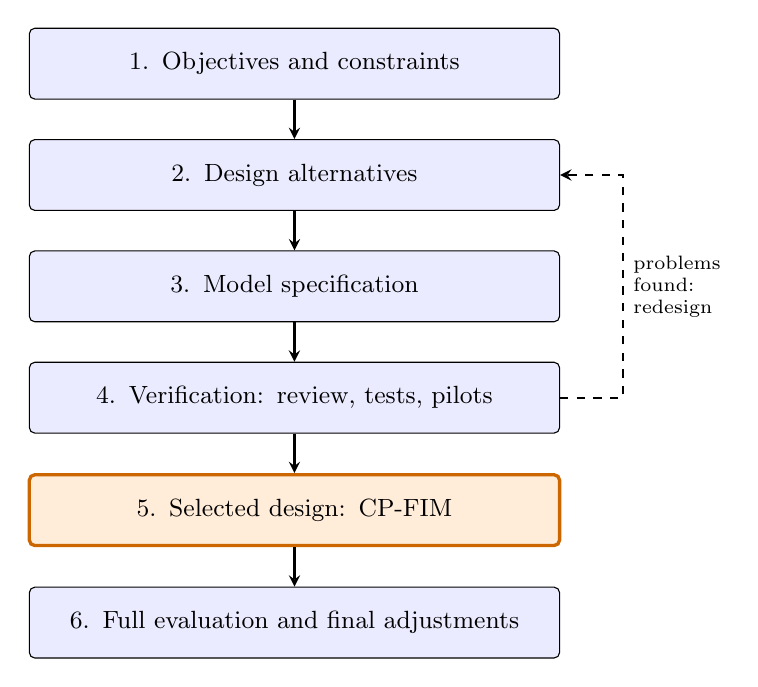
\begin{tikzpicture}[
    node distance=0.5cm,
    s/.style={rectangle, draw, rounded corners=2pt, fill=blue!8, text width=6.5cm, align=center, minimum height=0.9cm, font=\small},
    f/.style={rectangle, draw=orange!80!black, very thick, rounded corners=2pt, fill=orange!15, text width=6.5cm, align=center, minimum height=0.9cm, font=\small},
    arrow/.style={thick,->,>=stealth}]
    \node[s] (o) {1. Objectives and constraints};
    \node[s, below=of o] (a) {2. Design alternatives};
    \node[s, below=of a] (p) {3. Model specification};
    \node[s, below=of p] (v) {4. Verification: review, tests, pilots};
    \node[f, below=of v] (c) {5. Selected design: CP-FIM};
    \node[s, below=of c] (e) {6. Full evaluation and final adjustments};
    \draw[arrow] (o) -- (a); \draw[arrow] (a) -- (p); \draw[arrow] (p) -- (v); \draw[arrow] (v) -- (c); \draw[arrow] (c) -- (e);
    \draw[arrow, dashed] (v.east) -- ++(0.8,0) |- node[pos=0.25, right, font=\scriptsize, align=left]{problems\\found:\\redesign} (a.east);
\end{tikzpicture}

% 3. Geometry of the two-goal MGDA (Pareto) weight (Chapter 4)
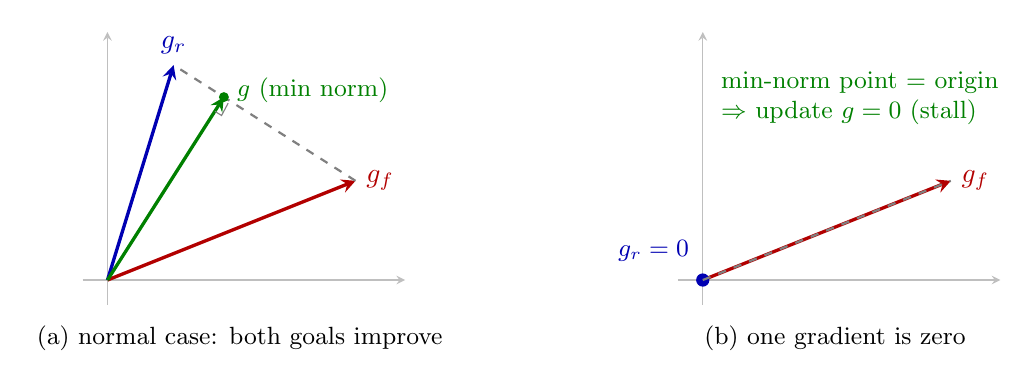
\begin{tikzpicture}[scale=1.05, >=stealth]
  \begin{scope}
    \draw[gray!50, ->] (-0.3,0) -- (3.6,0); \draw[gray!50, ->] (0,-0.3) -- (0,3.0);
    \draw[very thick, ->, red!70!black] (0,0) -- (3,1.2) node[right]{$g_f$};
    \draw[very thick, ->, blue!70!black] (0,0) -- (0.8,2.6) node[above]{$g_r$};
    \draw[thick, dashed, gray] (3,1.2) -- (0.8,2.6);
    \draw[very thick, ->, green!50!black] (0,0) -- (1.408,2.213);
    \fill[green!50!black] (1.408,2.213) circle (0.06);
    \node[green!50!black, right] at (1.45,2.30) {\small $g$ (min norm)};
    \draw[gray] (1.30,2.04) -- (1.38,1.99) -- (1.46,2.14);
    \node[font=\small] at (1.6,-0.7) {(a) normal case: both goals improve};
  \end{scope}
  \begin{scope}[xshift=7.2cm]
    \draw[gray!50, ->] (-0.3,0) -- (3.6,0); \draw[gray!50, ->] (0,-0.3) -- (0,3.0);
    \draw[very thick, ->, red!70!black] (0,0) -- (3,1.2) node[right]{$g_f$};
    \fill[blue!70!black] (0,0) circle (0.08);
    \node[blue!70!black, left] at (-0.05,0.35) {\small $g_r = 0$};
    \draw[thick, dashed, gray] (0,0) -- (3,1.2);
    \node[green!50!black, font=\small, align=left] at (1.9,2.2) {min-norm point = origin\\ $\Rightarrow$ update $g = 0$ (stall)};
    \node[font=\small] at (1.6,-0.7) {(b) one gradient is zero};
  \end{scope}
\end{tikzpicture}

% 4. Leakage control timeline (Chapter 4)
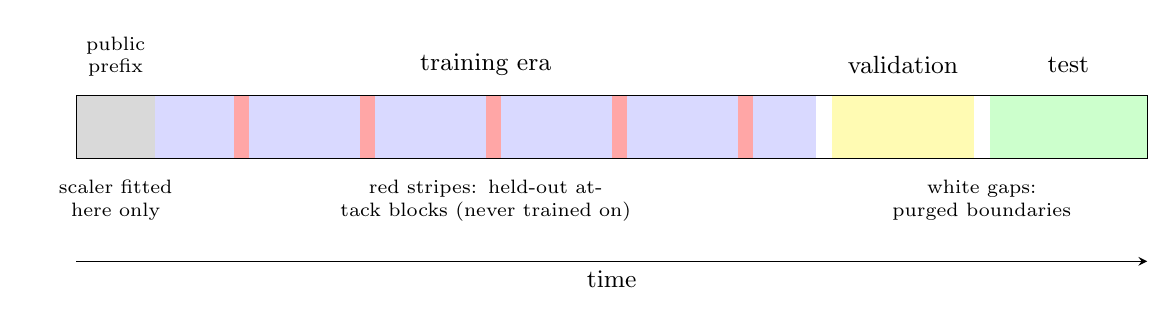
\begin{tikzpicture}[x=1cm, y=1cm]
  \fill[gray!30] (0,0) rectangle (1.0,0.8);
  \fill[blue!15] (1.0,0) rectangle (9.4,0.8);
  \fill[white] (9.4,0) rectangle (9.6,0.8);
  \fill[yellow!30] (9.6,0) rectangle (11.4,0.8);
  \fill[white] (11.4,0) rectangle (11.6,0.8);
  \fill[green!20] (11.6,0) rectangle (13.6,0.8);
  \foreach \x in {2.0, 3.6, 5.2, 6.8, 8.4} { \fill[red!35] (\x,0) rectangle (\x+0.2,0.8); }
  \draw (0,0) rectangle (13.6,0.8);
  \node[font=\scriptsize, align=center] at (0.5,1.3) {public\\ prefix};
  \node[font=\small] at (5.2,1.2) {training era};
  \node[font=\small] at (10.5,1.2) {validation};
  \node[font=\small] at (12.6,1.2) {test};
  \node[font=\scriptsize, text width=2.0cm, align=center, anchor=north] at (0.5,-0.15) {scaler fitted here only};
  \node[font=\scriptsize, text width=6.5cm, align=center, anchor=north] at (5.2,-0.15) {red stripes: held-out attack blocks (never trained on)};
  \node[font=\scriptsize, text width=3.6cm, align=center, anchor=north] at (11.5,-0.15) {white gaps: purged boundaries};
  \draw[->, >=stealth] (0,-1.3) -- (13.6,-1.3) node[midway, below, font=\small]{time};
\end{tikzpicture}

\end{document}
